\documentclass[12pt]{beamer}

%\usetheme{CambridgeUS}
\usetheme{Boadilla}
\setbeamertemplate{navigation symbols}{}
\setbeamertemplate{headline}{}
%\setbeamercovered{transparent}

\usepackage[british]{babel}
\usepackage[useregional]{datetime2}
\DTMlangsetup[en-GB]{showdayofmonth=false}

\usepackage[utf8]{inputenc}
\usepackage{derivative}
\usepackage{mathtools}

\title{Orbital Motion about a Black Hole}
\subtitle{ACM40980 Presentation}
\author[Karl Coogan]{Karl Coogan\\[10mm]{Supervisor: Dr. Niels Warburton}}
\date{\today}

\begin{document}

\maketitle

\begin{frame}{Agenda}
\begin{itemize}
    \item Introduction to General Relativity
    \item Schwarzschild Black Holes
    \item Kerr Black Holes
    \item \alert<2>{Resonant Orbits}
\end{itemize}
\end{frame}

\begin{frame}{Introduction to General Relativity}{In the beginning\ldots}
\begin{itemize}
    \item[] Newton's Law of Universal Gravitation (1687)
    \begin{itemize}
        \item Every particle in the universe attracts every other particle.
    \end{itemize}
    \item[]
    \item[] Einstein's Theory of Special Relativity (1907)
    \begin{itemize}
        \item The motion of one object is always relative to the motion of another object.
    \end{itemize}
    \item[]
    \item[] Einstein's Theory of General Relativity (1915)
    \begin{itemize}
        \item Gravitation can be thought of as a curved field, instead of a force.
    \end{itemize}
\end{itemize}
\end{frame}

\begin{frame}{Introduction to General Relativity}{Metrics and the Einstein Field Equations}
From general relativity came the Einstein Field Equations
\begin{equation}
    G_{ab}+\Lambda g_{ab}=\frac{8\pi G}{c^4}T_{ab}.
\end{equation}
This relates the geometry of spacetime to the distribution of matter within it.\\
\vskip10pt
Exact solutions to these equations are called metrics.
\end{frame}

\begin{frame}{Schwarzschild Black Holes}{History \& Properties}
\begin{columns}
\column{0.5\textwidth}
The Schwarzschild metric was discovered in 1916 by Karl Schwarzschild.\\
\vskip10pt
A good starting point for understanding orbital motion, primarily because of the following two properties:
\vskip10pt
\begin{itemize}
    \item \alert<2>{No angular momentum}
    \item No electrical charge 
\end{itemize}

\column{0.5\textwidth}
\begin{center}
    \includegraphics<1>[width=\textwidth]{SchwarzOrbitNonEcc.pdf}
    \includegraphics<2>[width=\textwidth]{SchwarzOrbitEcc.pdf}
\end{center}

\end{columns}
\end{frame}

\begin{frame}{Schwarzschild Black Holes}{The Schwarzschild Metric}
Before we move on, we first define the Schwarzschild metric as
\begin{equation}
g_{\alpha\beta}=
\begin{pmatrix}
    -f(r) & 0 & 0 & 0\\
    0 & f(r)^{-1} & 0 & 0\\
    0 & 0 & r^2 & 0\\
    0 & 0 & 0 & r^2\sin(\theta)
\end{pmatrix},
\end{equation}
where we note that only the non-zero entries are along the diagonal, also we define
\begin{equation}
f(r)=\frac{r-2M}{r}.
\end{equation}
\end{frame}

\begin{frame}{Schwarzschild Black Holes}{Orbital Motion: Two Ways}
\begin{columns}[c]
\begin{column}{0.5\textwidth}
\centering
Euler-Lagrange Equation
$$\odv{}{\tau}\left(\pdv{\mathcal{L}}{u^\alpha}\right)=\pdv{\mathcal{L}}{x^\alpha}$$
\begin{itemize}
    \item We know there are constants because of Noether's Theorem
\end{itemize}
\end{column}
\vrule{}
\begin{column}{0.5\textwidth}
\centering
Geodesic Equation
$$\odv[order=2]{x^\alpha}{\lambda} + \Gamma^t{}_{\beta\delta}\odv{x^\beta}{\lambda}\odv{x^\delta}{\lambda}=0$$
\begin{itemize}
    \item This is the most straightforward way to solve for the motion of a particle
\end{itemize}
\end{column}
\end{columns}
\end{frame}

\begin{frame}{Schwarzschild Black Holes}{Orbital Motion: Results}
\centering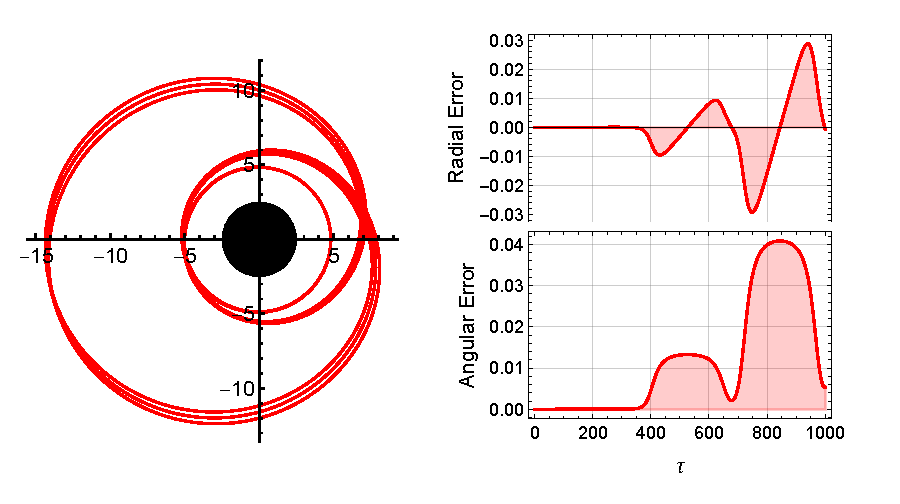
\includegraphics[width=\textwidth]{MatchedOrbits.pdf}
\end{frame}

\begin{frame}{Schwarzschild Black Holes}{Bound Orbits}
\centering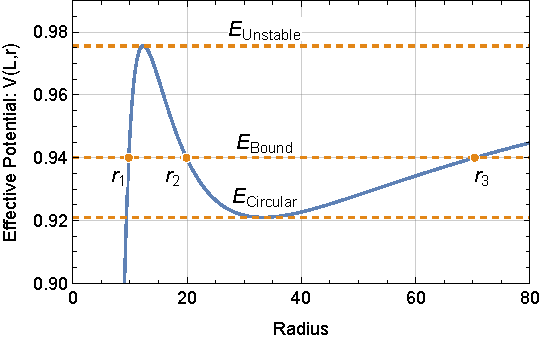
\includegraphics[width=0.85\textwidth]{RadialPotentialPE.pdf}
\end{frame}

\begin{frame}{Kerr Black Holes}{History \& Properties}
\begin{columns}
\column{0.5\textwidth}
The Kerr metric was discovered in 1963 by Roy Kerr.\\
\vskip10pt
It describes the geometry about uncharged black holes with \alert<2>{non-zero angular momentum}.
\vskip10pt
We now take an interest in \alert<3>{orbits outside the equatorial plane}.

\column{0.5\textwidth}
\centering
\begin{center}
    \includegraphics<1>[width=\textwidth]{kerrExample1.pdf}
    \includegraphics<2>[width=\textwidth]{kerrExample2.pdf}
    \includegraphics<3>[width=\textwidth]{kerrExample3.pdf}
\end{center}

\end{columns}
\end{frame}

\begin{frame}{Kerr Black Holes}{The Kerr Metric}
Let us now define the line element of the Kerr metric:
\begin{equation}
\begin{split}
\odif{s}^2&=-\left(1-\frac{2Mr}{\Sigma} \right)\odif{t}^2 + \frac{\Sigma}{\Delta}\odif{r}^2 +\Sigma\odif{\theta}^2\\
&\qquad+\left(r^2+a^2+\frac{2Ma^2r\sin^2(\theta)}{\Sigma}\right)\sin^2(\theta)\odif{\phi}^2\\
&\qquad- \frac{4Mar\sin^2(\theta)}{\Sigma}\odif{t}\odif{\phi},
\end{split}
\end{equation}
where
\begin{gather}
\Delta=r^2-2Mr+a^2,\\
\Sigma=r^2+a^2\cos(\theta).
\end{gather}
\end{frame}

\begin{frame}{Kerr Black Holes}{Orbital Frequencies}
As bound Kerr orbits are triperiodic, there are three frequencies that we can examine.
\vskip10pt
\begin{itemize}
    \item[] \alert<2->{$\Upsilon_r$: Radial oscillations}
    \item[] \alert<2->{$\Upsilon_\theta$: Polar oscillations}
    \item[] $\Upsilon_\phi$: Rotations about the black hole's axis of spin
\end{itemize}
\end{frame}

\begin{frame}{Resonant Orbits}{Definition}
Resonant orbits occur when the following equation is satisfied
\begin{equation}
	k\Upsilon_\theta=n\Upsilon_r,
\end{equation}
where $k$ and $n$ are two relatively prime integers.
\vskip12pt
It says that it takes an equal amount of time for the polar motion to pass through $k$
turning points as it does for the radial motion to pass through $n$ turning points.
\end{frame}

\begin{frame}{Resonant Orbits}{Example}
An example of a $(k,n)=(2,3)$ resonant orbit is shown below
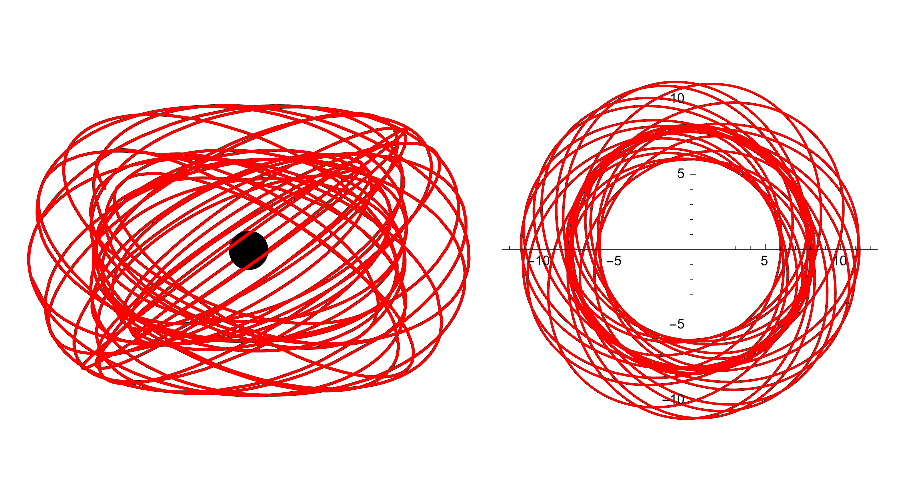
\includegraphics[width=\textwidth]{kerrResoExample23.pdf}
\end{frame}

\begin{frame}{Resonant Orbits}{$(r,\cos(\theta))$ Plot}
    \centering
    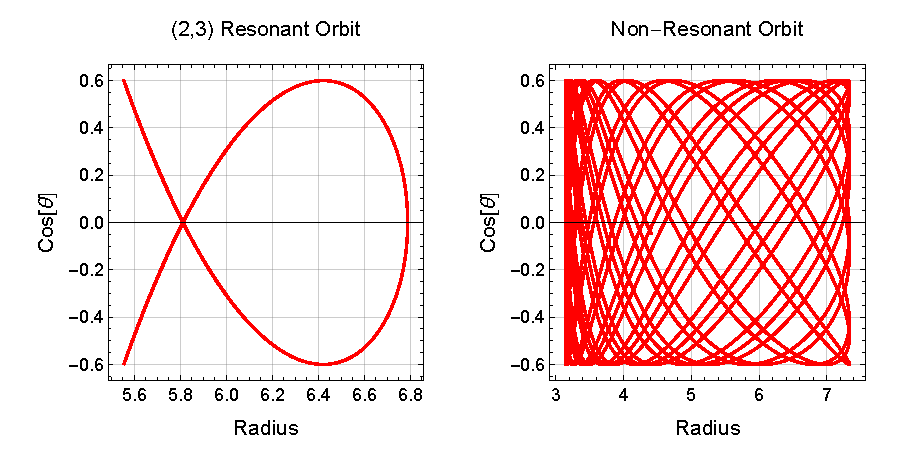
\includegraphics[width=\textwidth]{kerrRThReso.pdf}
\end{frame}

\begin{frame}{Resonant Orbits}{Perturbations and Long Timeframes}
    \centering
    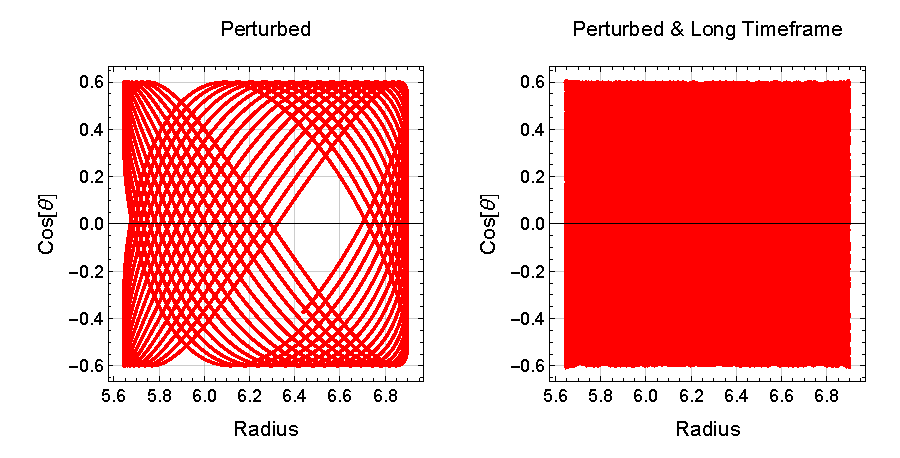
\includegraphics[width=\textwidth]{kerrRThResoLong.pdf}
\end{frame}

\begin{frame}{Resonant Orbits}{A Strange Observation}
Setting the spin of the black hole, $a$, to $0.9$, the following plot was produced which shows the plane of all resonant $(p,e,x)$\footnote{\textbf{Note:} $p$ is the size of the orbit, $e$ is the eccentricity, and $x$ is the inclination angle from the equatorial plane.} values for $(2,3)$-type resonances.

\centering
    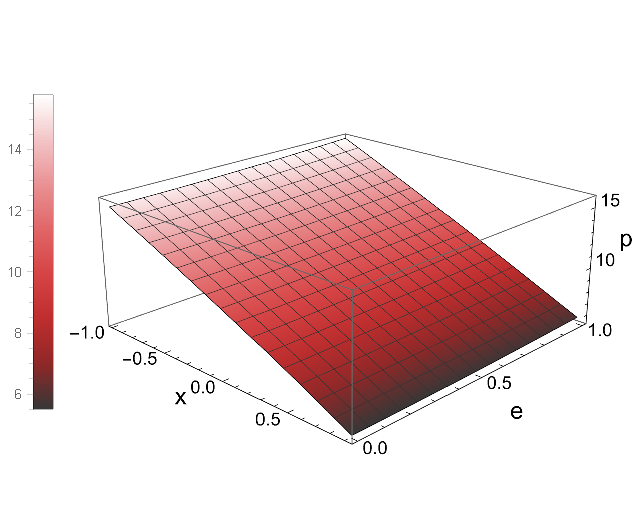
\includegraphics[width=0.54\textwidth]{resoPEXPlane.pdf}
\end{frame}

\begin{frame}{Resonant Orbits}{Root-Finding: Creating a Plane of Initial Values}
We want to develop a way to estimate these resonant $p$ values, so we set $e=0$ and solve the equation
\begin{equation}
	2\Upsilon_\theta=3\Upsilon_r
\end{equation}
for $p$ when $x=+1$ and $x=-1$.
\vskip12pt
This will allow us to create a line in the $(p,x)$ plane at $e=0$ and then extrapolate out for $0<e\leq 1$.
\end{frame}

\begin{frame}{Resonant Orbits}{Root-Finding: The Equations to be Solved}
\centering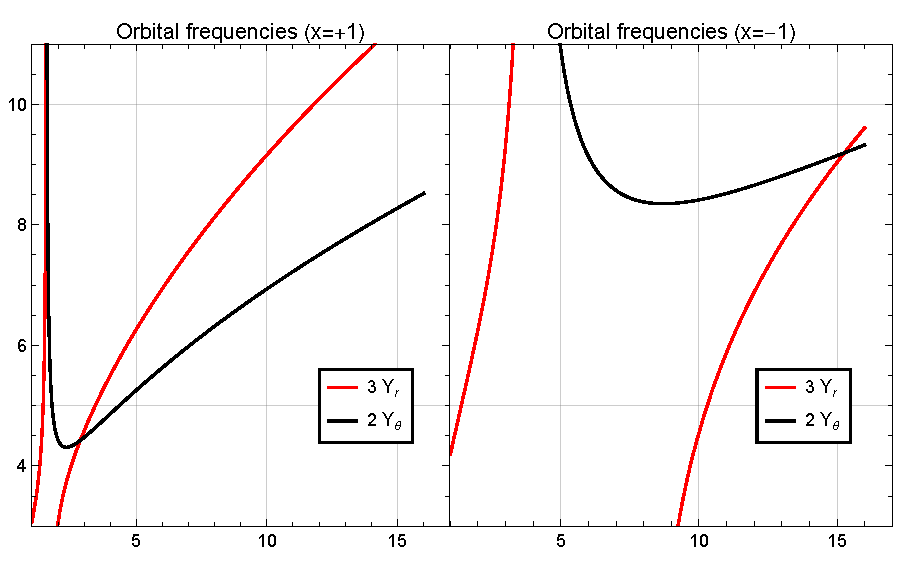
\includegraphics[width=0.9\textwidth]{proretfreqplots.pdf}
\end{frame}

\begin{frame}{Resonant Orbits}{Root-Finding: The Results}
	Solving for the points of intersection in the previous plots gives us
	\begin{equation}
		p_{x=+1}=4.9626,\qquad p_{x=-1}=15.2677.
	\end{equation}
	We now calculate the equation for the line between the two points $(+1,4.9626)$ and $(-1,15.2677)$, which gives us
	\begin{equation}
	f(x)=10.1152-5.1525x.
\end{equation}	 
Finally, we extend this line out to a plane for $0<e\leq 1$:
\begin{equation}
	f(e,x)=10.1152-5.1525x+e.
\end{equation}	 
\end{frame}

\begin{frame}{Resonant Orbits}{Root-Finding: Error Compared to True Values}
\centering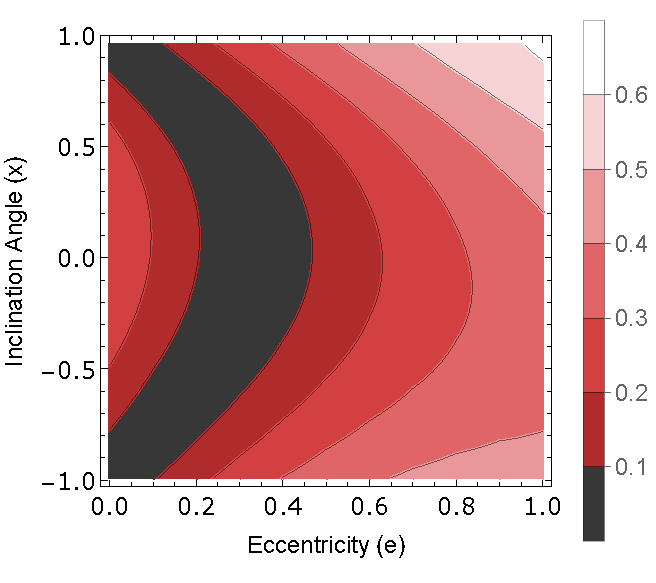
\includegraphics[width=0.6\textwidth]{errorContour.pdf}
\end{frame}

\begin{frame}
\begin{center}
\Large{Thank you all for coming,\\
I am happy to answer any questions.}
\end{center}
\end{frame}

\end{document}
